\section{appendix}
\label{sec:appendix}
\begin{figure}[H]
    \centering
    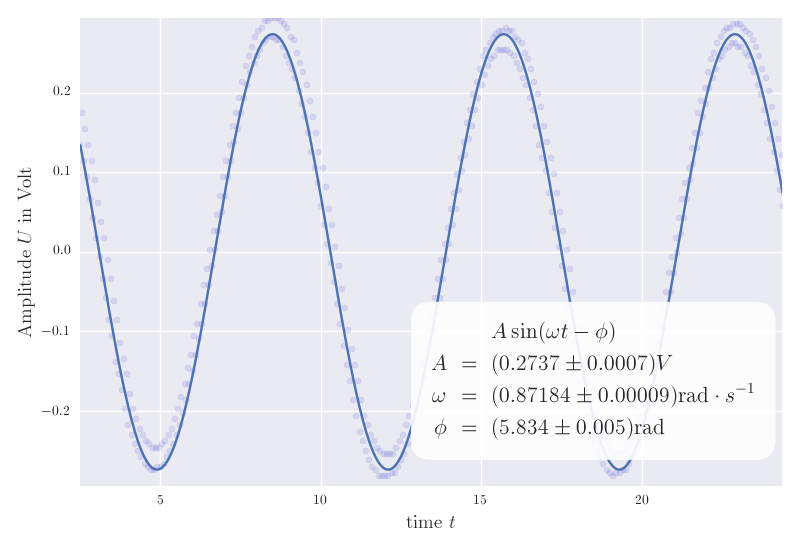
\includegraphics[width=0.7\linewidth]{analysis/figures/fit4_1}
    \caption{Measurement 4.1: resistor R1 with corresponding least squares fit.}
    \label{fig:4_1_plot}
\end{figure}
\begin{figure}[H]
    \centering
    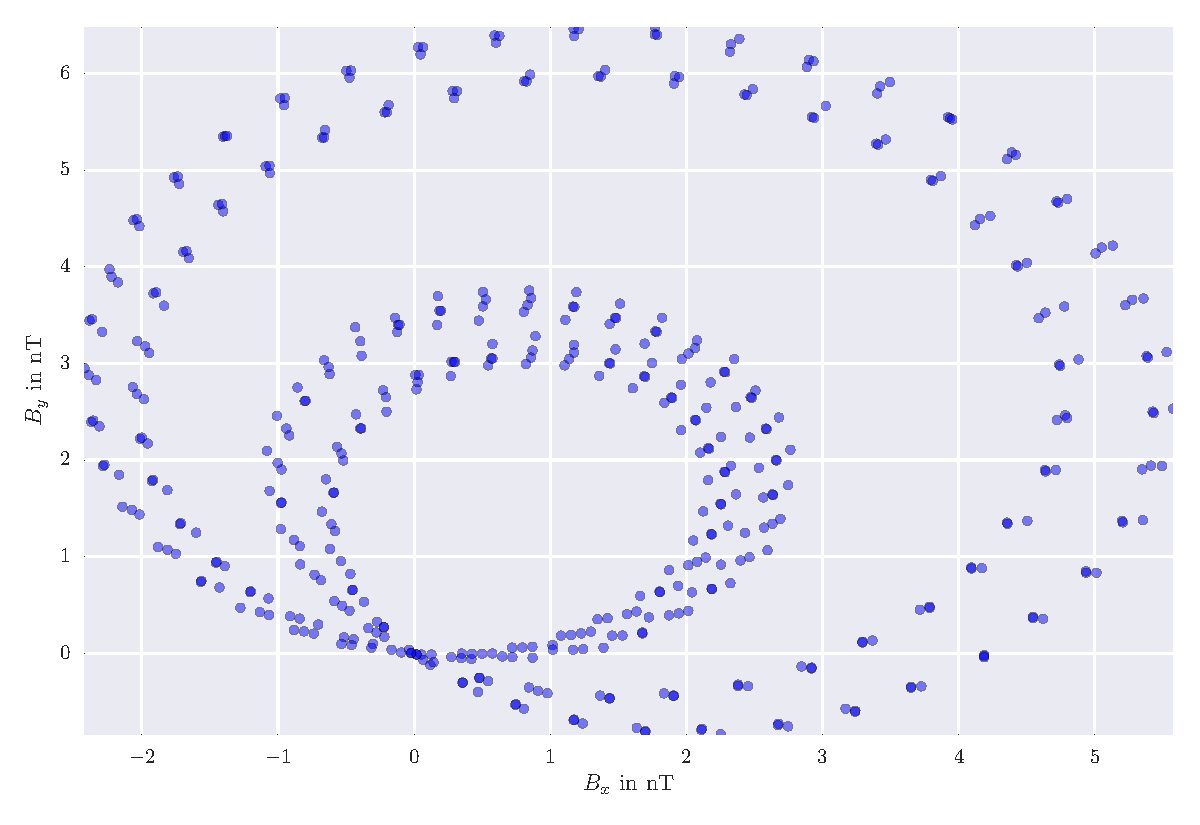
\includegraphics[width=0.7\linewidth]{analysis/figures/polar4_1}
    \caption{Measurement 4.1: Polarplot}
    \label{fig:4_1_polar}
\end{figure}

\begin{figure}[H]
    \centering
    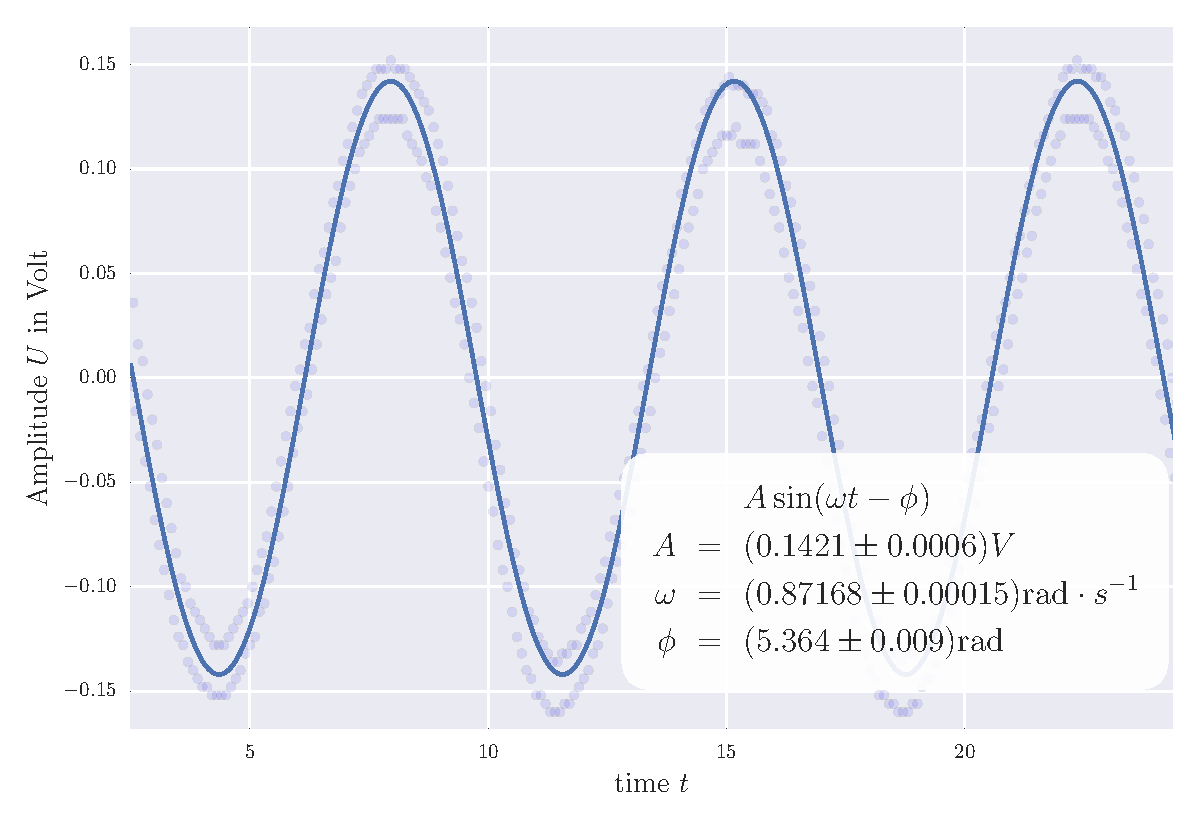
\includegraphics[width=0.7\linewidth]{analysis/figures/fit4_2}
    \caption{Measurement 4.2: resistor R2 with corresponding least squares fit.}
    \label{fig:4_2_plot}
\end{figure}
\begin{figure}[H]
    \centering
    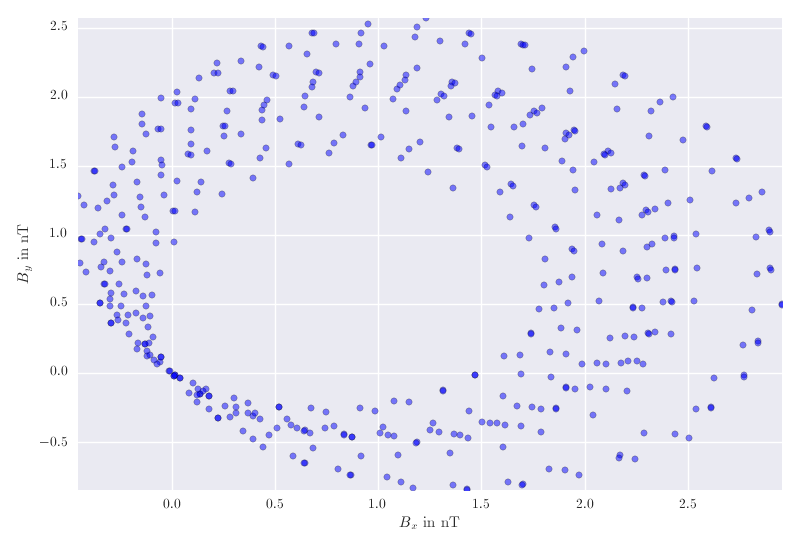
\includegraphics[width=0.7\linewidth]{analysis/figures/polar4_2}
    \caption{Measurement 4.2: Polarplot}
    \label{fig:4_2_polar}
\end{figure}

\begin{figure}[H]
    \centering
    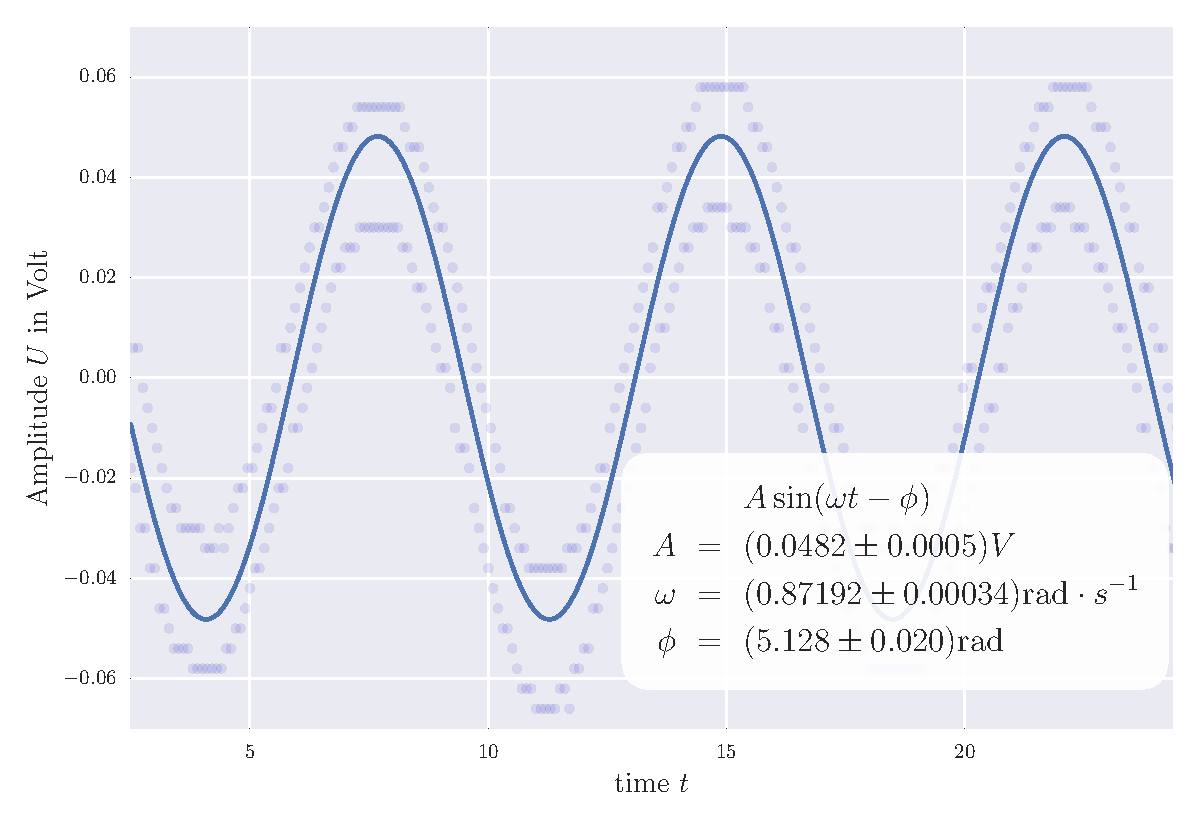
\includegraphics[width=0.7\linewidth]{analysis/figures/fit4_3}
    \caption{Measurement 4.3: resistor R3 with corresponding filtered data curve.}
    \label{fig:4_3_plot}
\end{figure}
\begin{figure}[H]
    \centering
    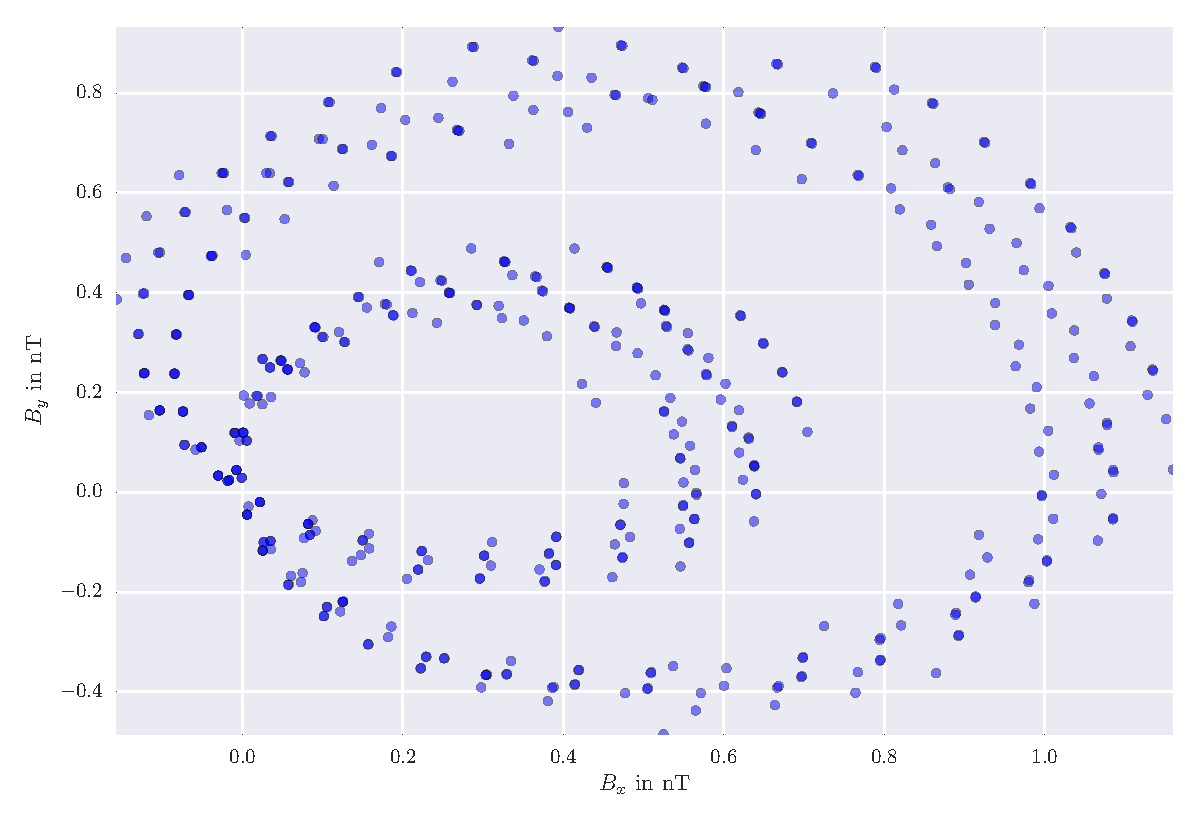
\includegraphics[width=0.7\linewidth]{analysis/figures/polar4_3}
    \caption{Measurement 4.3: Polarplot}
    \label{fig:4_3_polar}
\end{figure}

\begin{figure}[H]
    \centering
    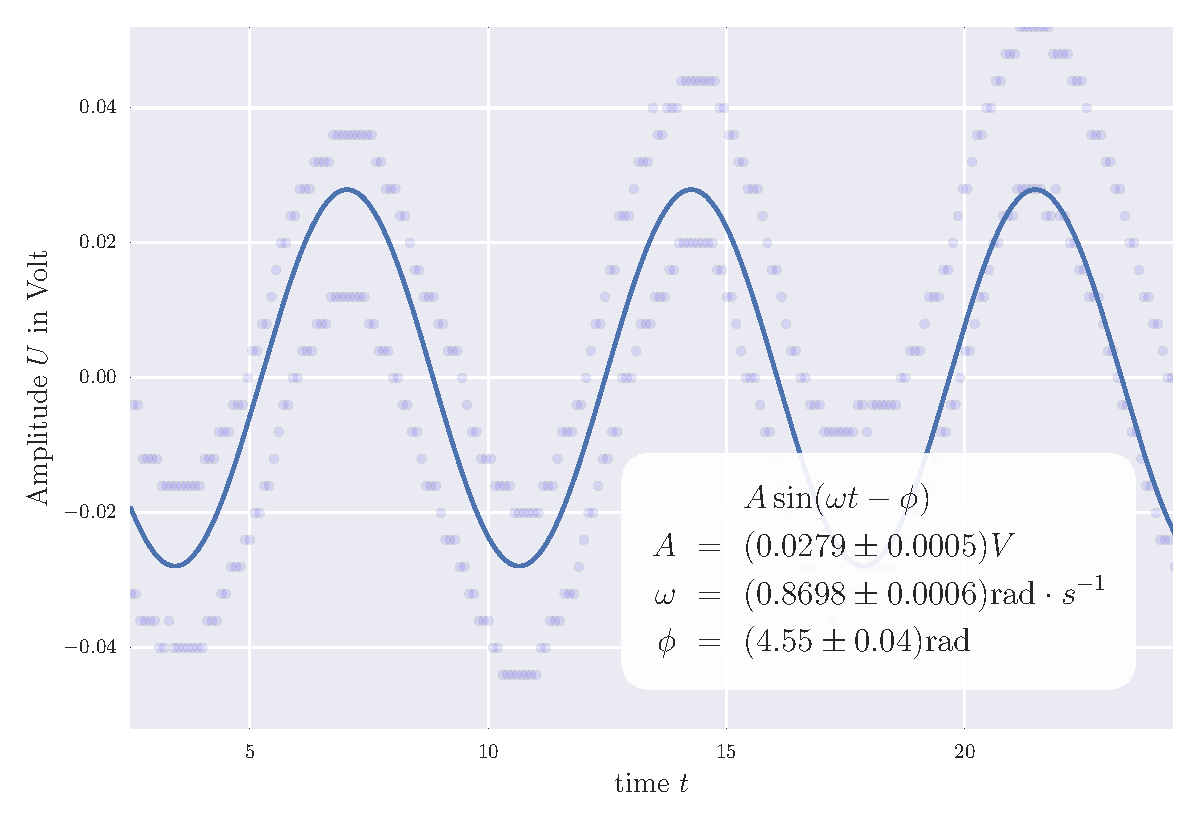
\includegraphics[width=0.7\linewidth]{analysis/figures/fit4_4}
    \caption{Measurement 4.4: resistor R4 with corresponding filtered data curve.}
    \label{fig:4_4_plot}
\end{figure}
\begin{figure}[H]
    \centering
    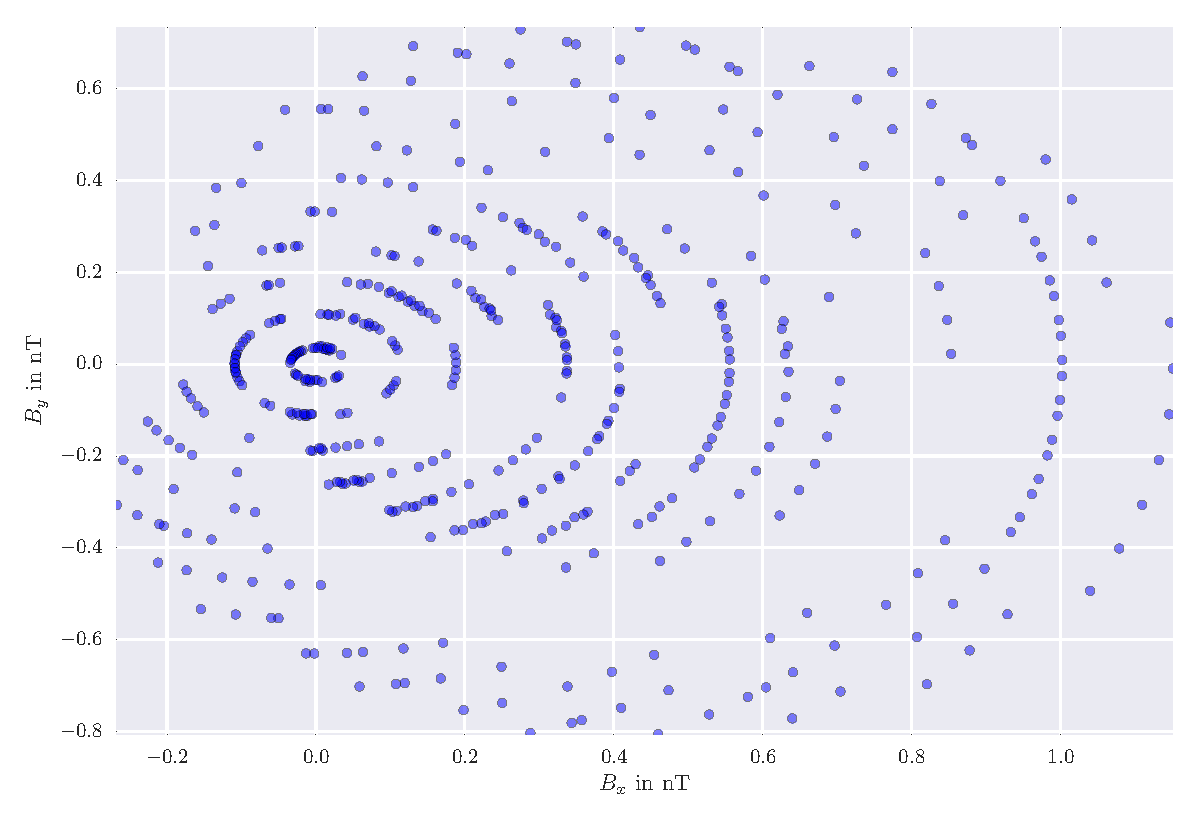
\includegraphics[width=0.7\linewidth]{analysis/figures/polar4_4}
    \caption{Measurement 4.4: Polarplot}
    \label{fig:4_4_polar}
\end{figure}

\begin{figure}[H]
    \centering
    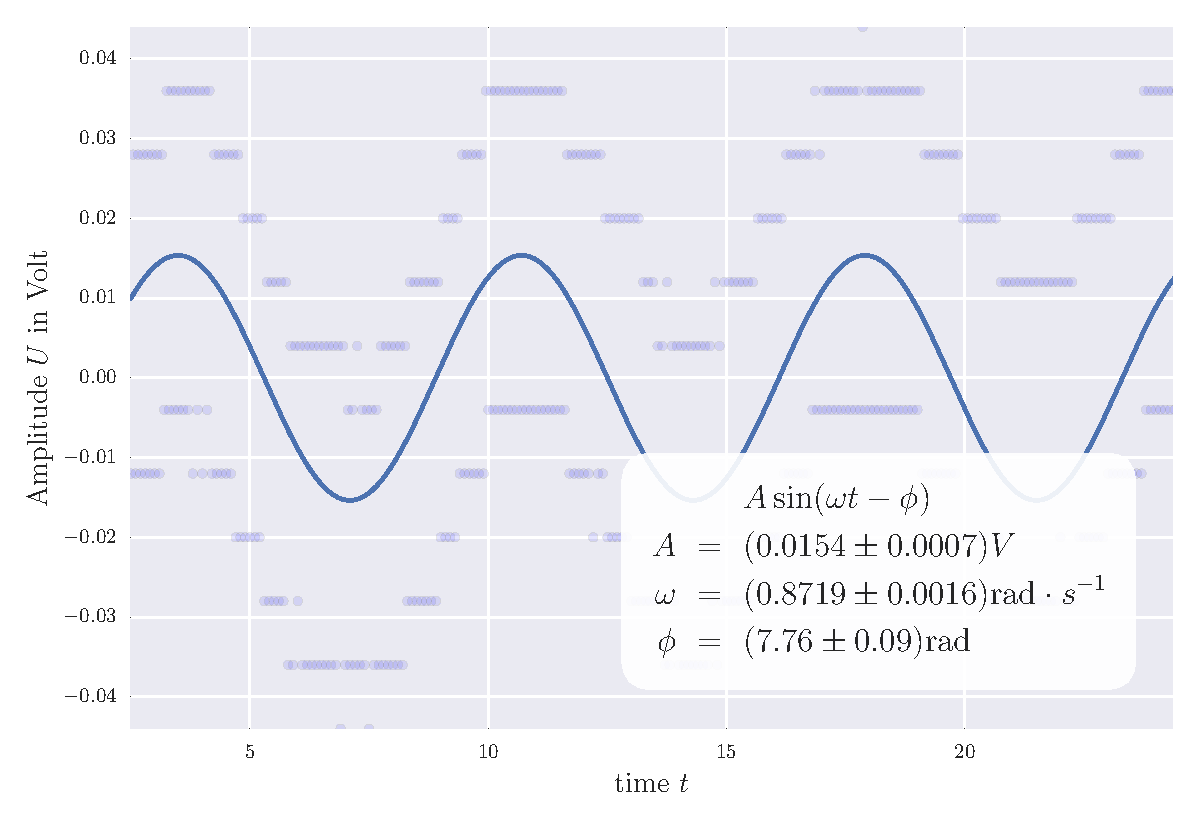
\includegraphics[width=0.7\linewidth]{analysis/figures/fit4_5}
    \caption{Measurement 4.5: resistor R5 with corresponding filtered data curve.}
    \label{fig:4_5_plot}
\end{figure}
\begin{figure}[H]
    \centering
    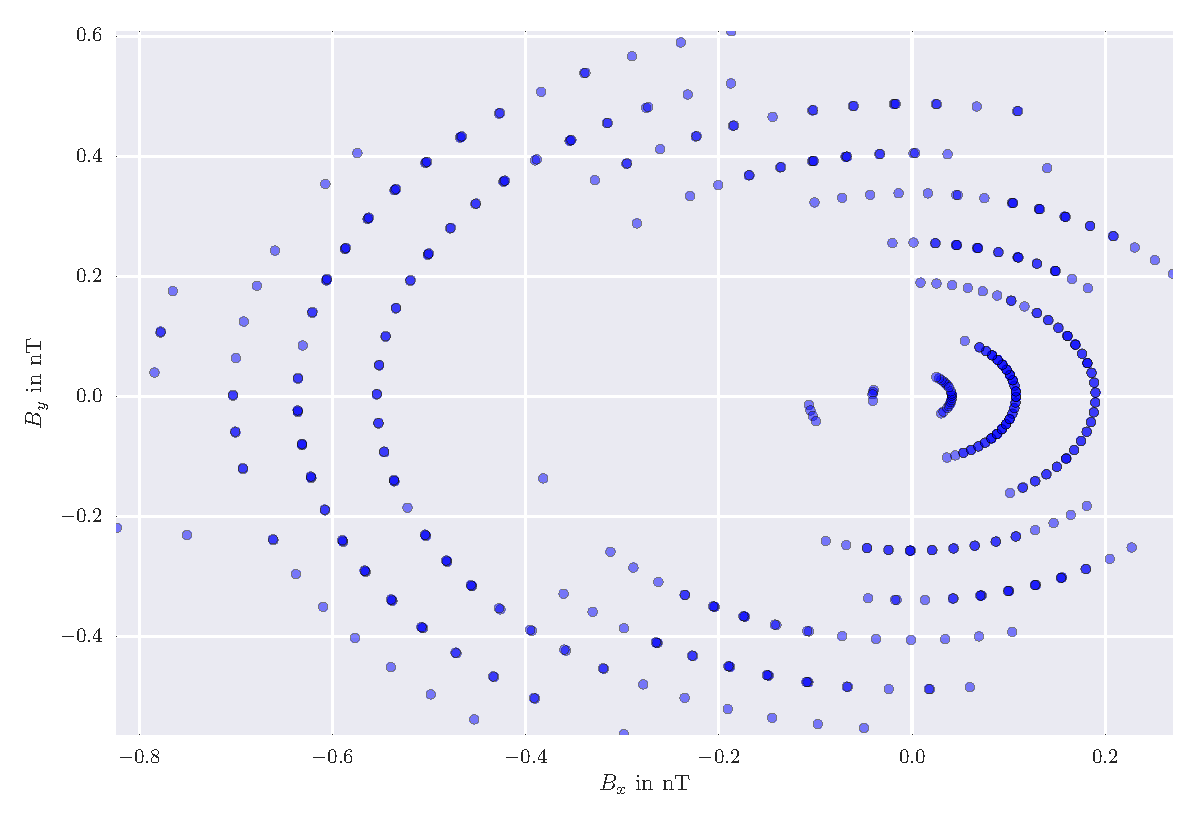
\includegraphics[width=0.7\linewidth]{analysis/figures/polar4_5}
    \caption{Measurement 4.5: Polarplot}
    \label{fig:4_5_polar}
\end{figure}

\begin{figure}[H]
    \centering
    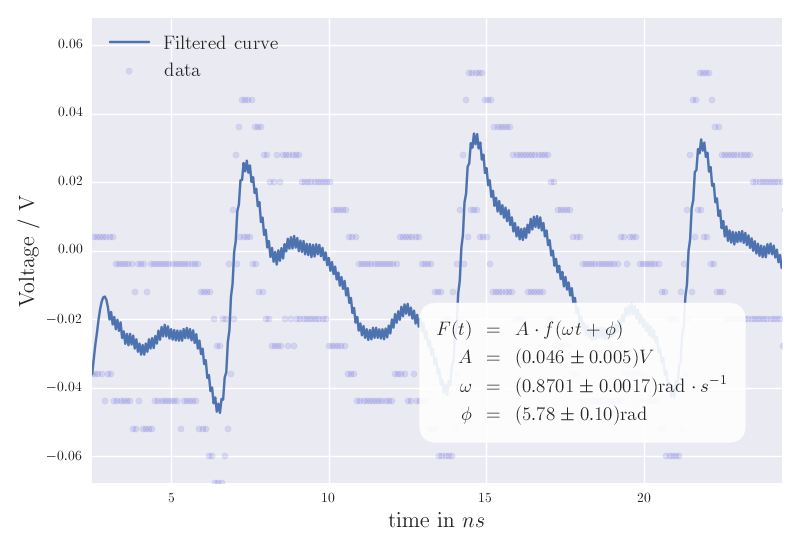
\includegraphics[width=0.7\linewidth]{analysis/figures/fit5_1}
    \caption{Measurement 5.1 (Gold) with corresponding filtered data curve.}
    \label{fig:5_1_plot}
\end{figure}
\begin{figure}[H]
    \centering
    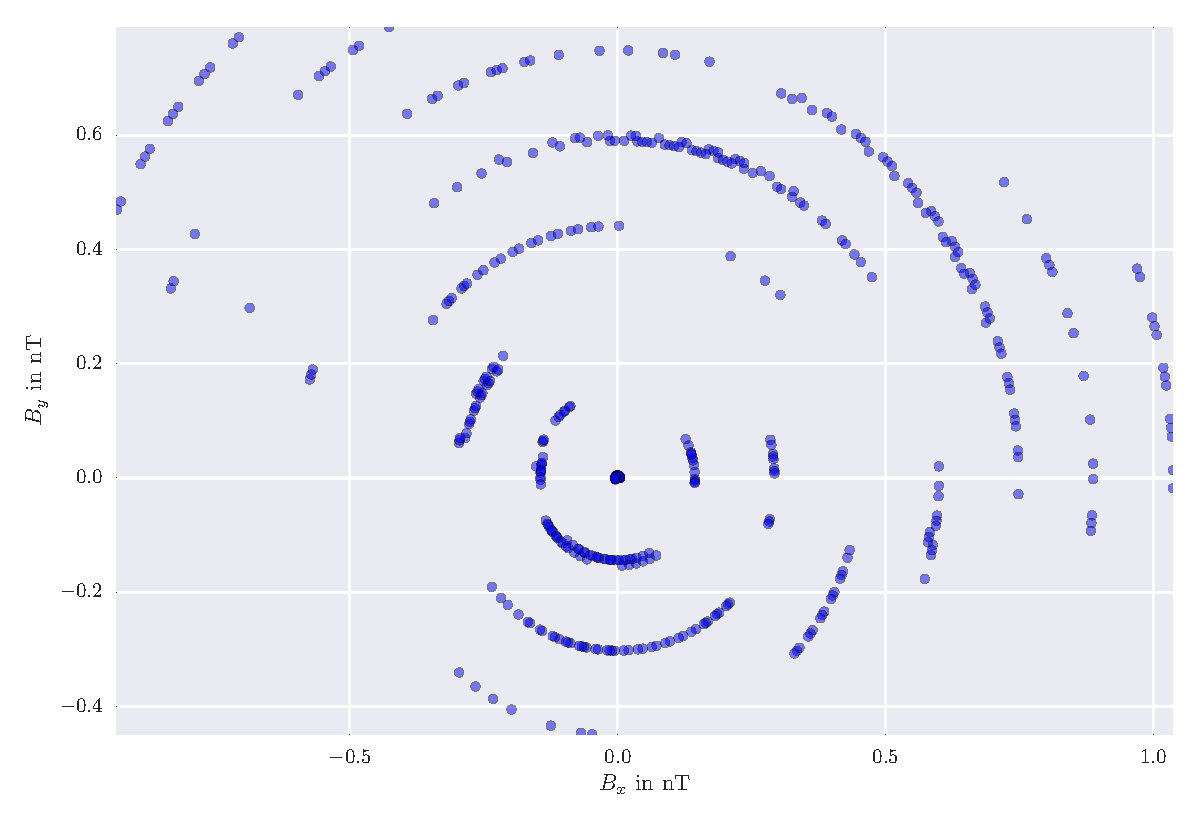
\includegraphics[width=0.7\linewidth]{analysis/figures/polar5_1}
    \caption{Measurement 5.1: Polarplot}
    \label{fig:5_1_polar}
\end{figure}

\begin{figure}[H]
    \centering
    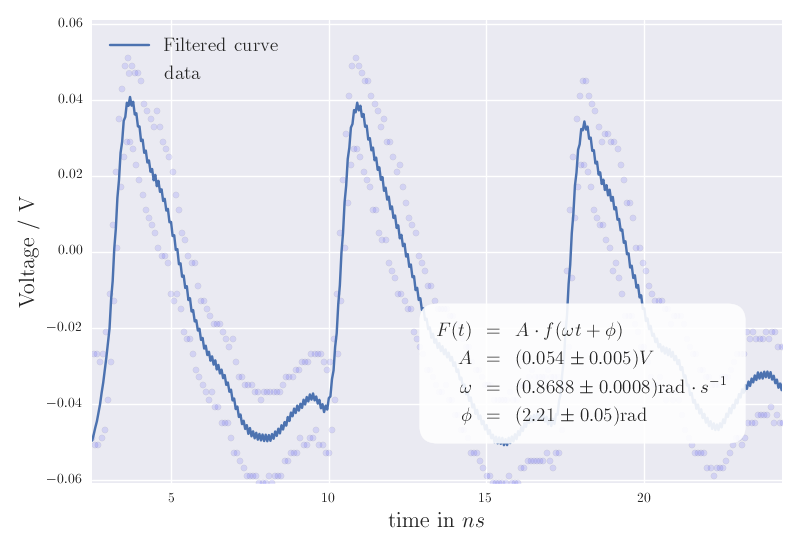
\includegraphics[width=0.7\linewidth]{analysis/figures/fit5_2}
    \caption{Measurement 5.2 (Iron) with corresponding filtered data curve.}
    \label{fig:5_2_plot}
\end{figure}
\begin{figure}[H]
    \centering
    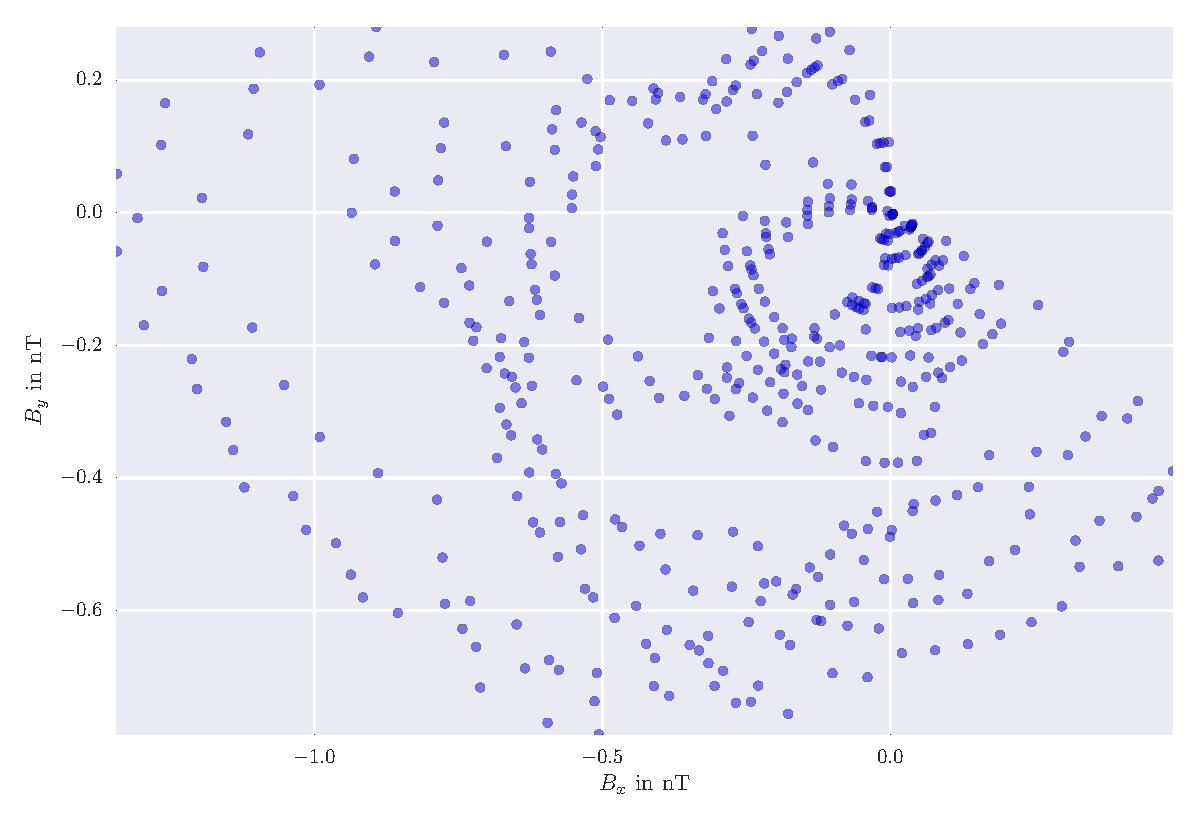
\includegraphics[width=0.7\linewidth]{analysis/figures/polar5_2}
    \caption{Measurement 5.2: Polarplot}
    \label{fig:5_2_polar}
\end{figure}

\begin{figure}[H]
    \centering
    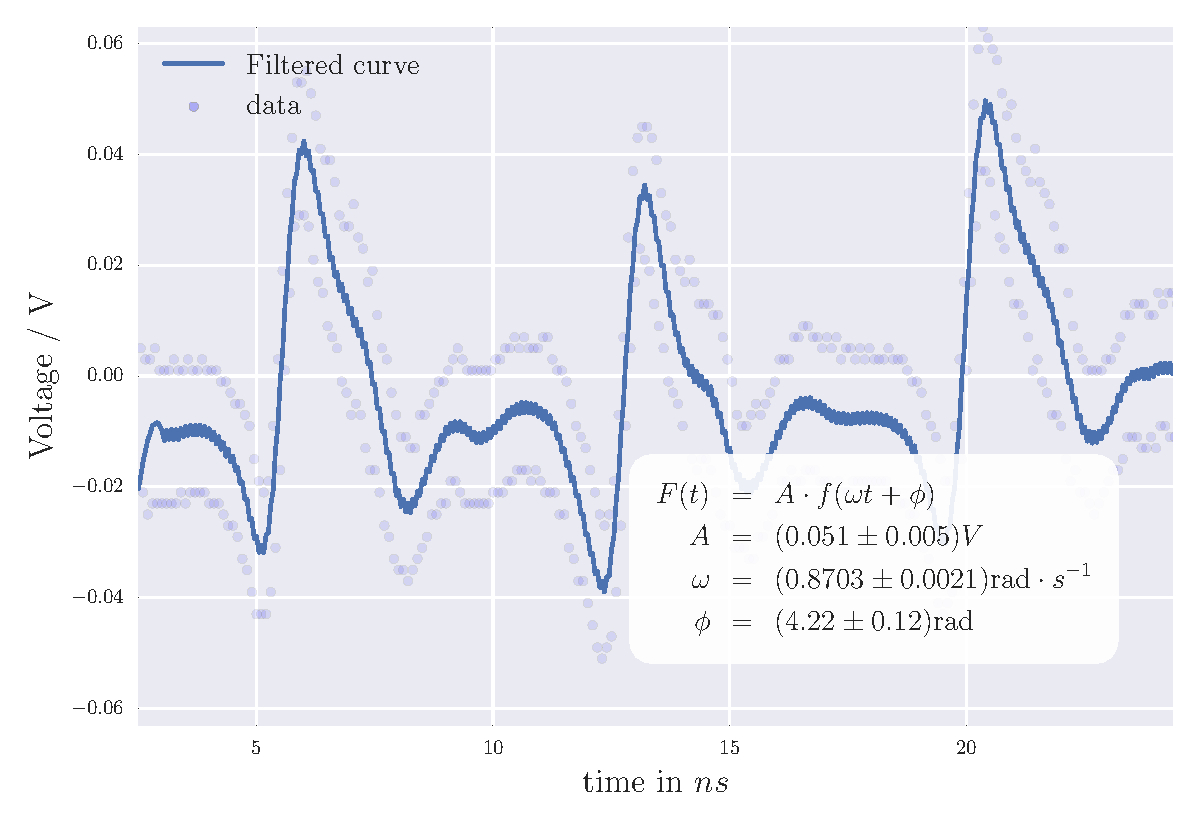
\includegraphics[width=0.7\linewidth]{analysis/figures/fit5_3}
    \caption{Measurement 5.3 (Stick) with corresponding least squares fit.}
    \label{fig:5_3_plot}
\end{figure}
\begin{figure}[H]
    \centering
    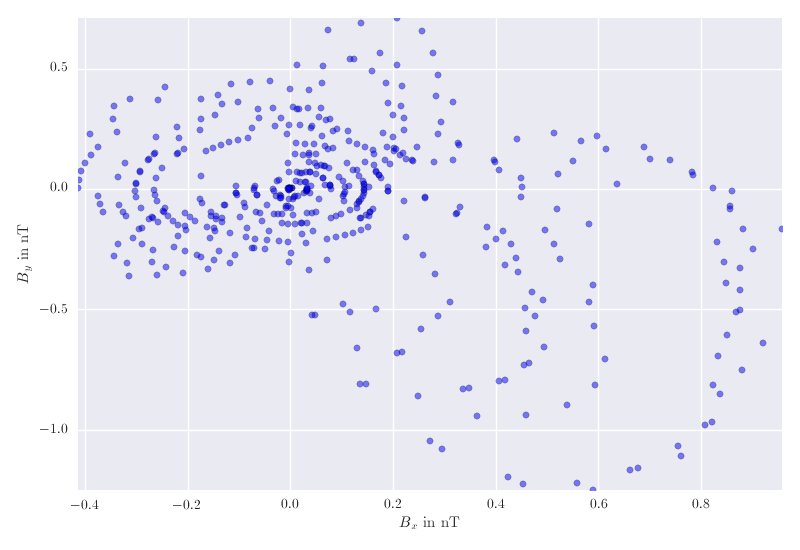
\includegraphics[width=0.7\linewidth]{analysis/figures/polar5_3}
    \caption{Measurement 5.3: Polarplot}
    \label{fig:5_3_polar}
\end{figure}

\begin{figure}[H]
    \centering
    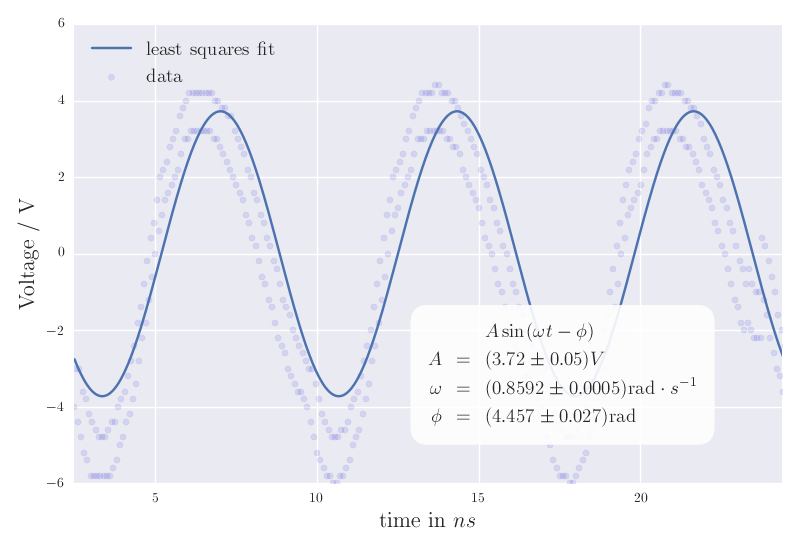
\includegraphics[width=0.7\linewidth]{analysis/figures/fit5_4}
    \caption{Measurement 5.4 (Magnetic splint) with corresponding least squares fit.}
    \label{fig:5_4_plot}
\end{figure}
\begin{figure}[H]
    \centering
    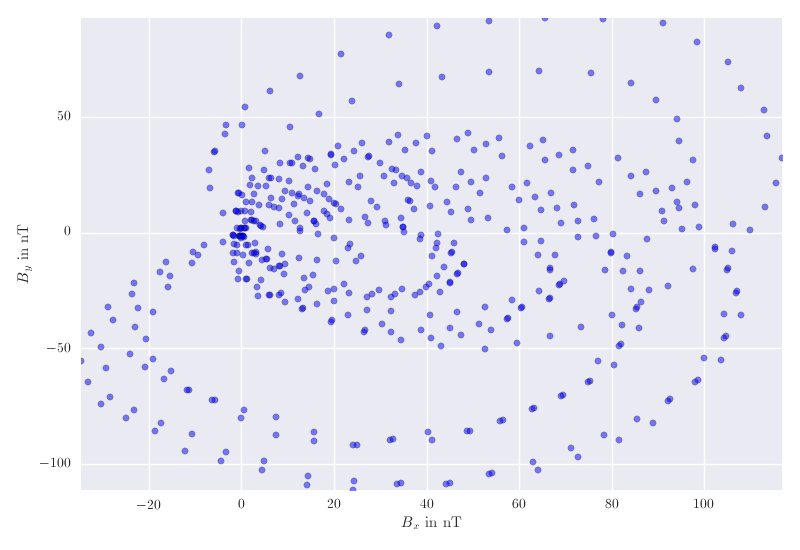
\includegraphics[width=0.7\linewidth]{analysis/figures/polar5_4}
    \caption{Measurement 5.4: Polarplot}
    \label{fig:5_4_polar}
\end{figure}

\begin{figure}[H]
    \centering
    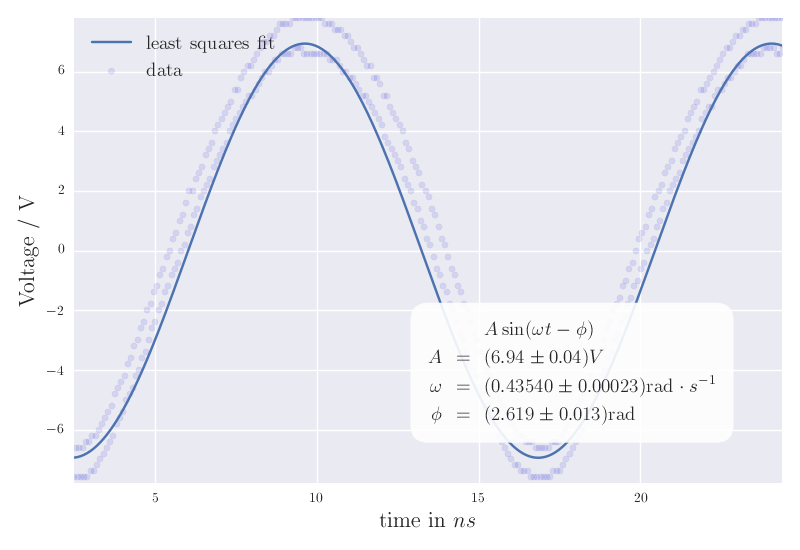
\includegraphics[width=0.7\linewidth]{analysis/figures/fit5_5}
    \caption{Measurement 5.5. with corresponding least squares fit.}
    \label{fig:5_5_plot}
\end{figure}
\begin{figure}[H]
    \centering
    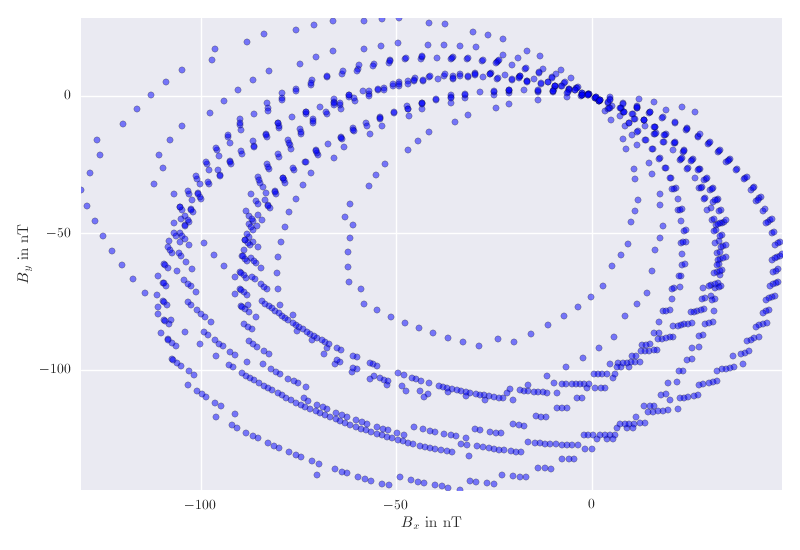
\includegraphics[width=0.7\linewidth]{analysis/figures/polar5_5}
    \caption{Measurement 5.5: Polarplot}
    \label{fig:5_5_polar}
\end{figure}

\subsection{Appendix: Handwritten records of the experiment}
\label{sec:records}
    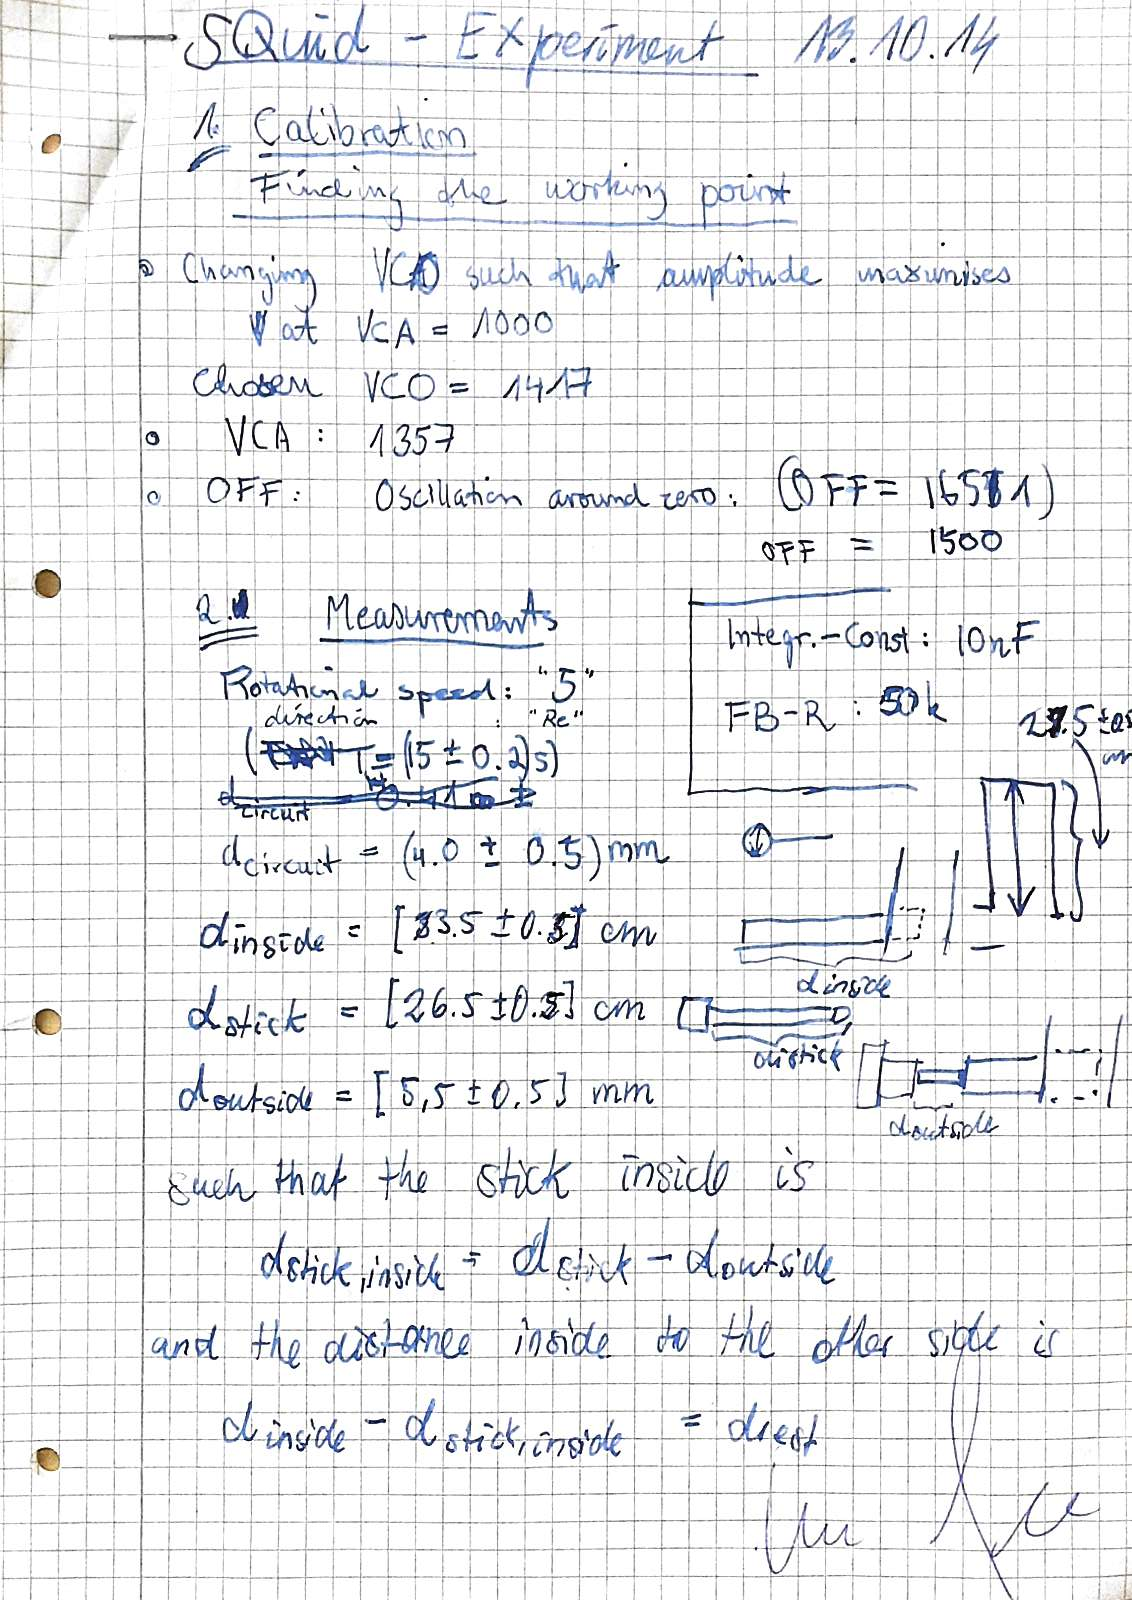
\includegraphics[width=\linewidth]{appendix/page1.jpeg}
    \clearpage
    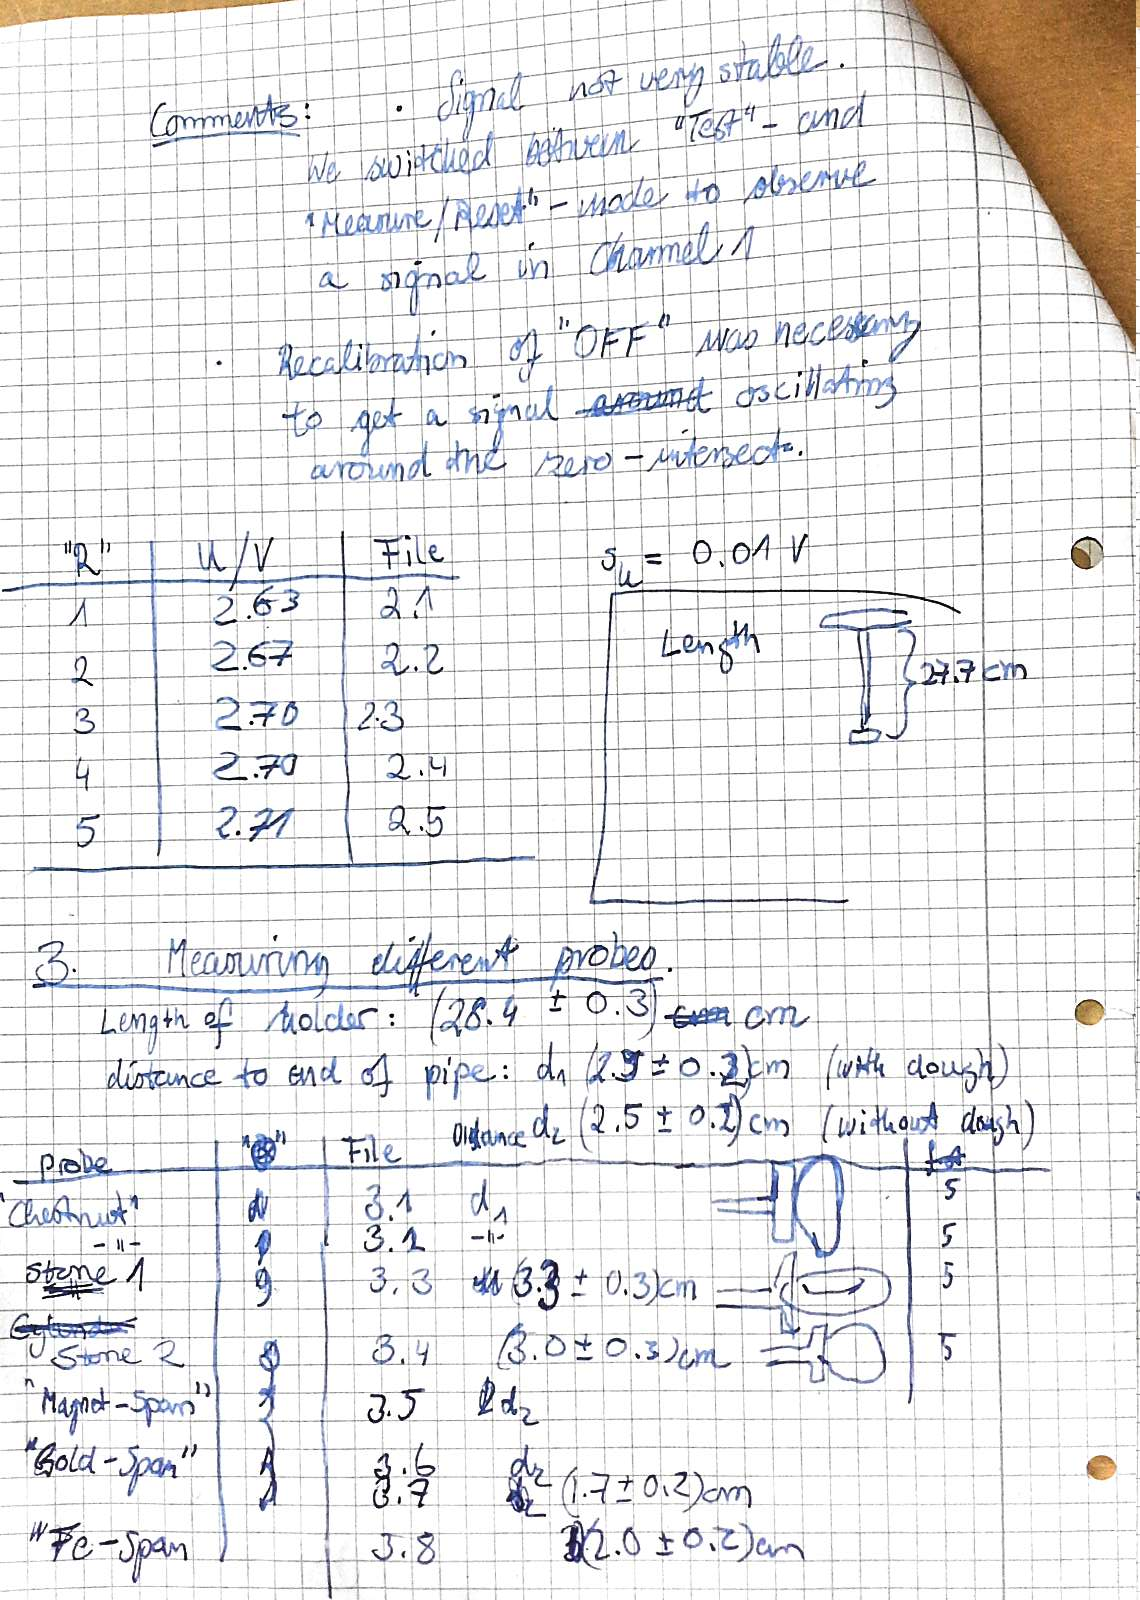
\includegraphics[width=\linewidth]{appendix/page2.jpeg}
    \clearpage
    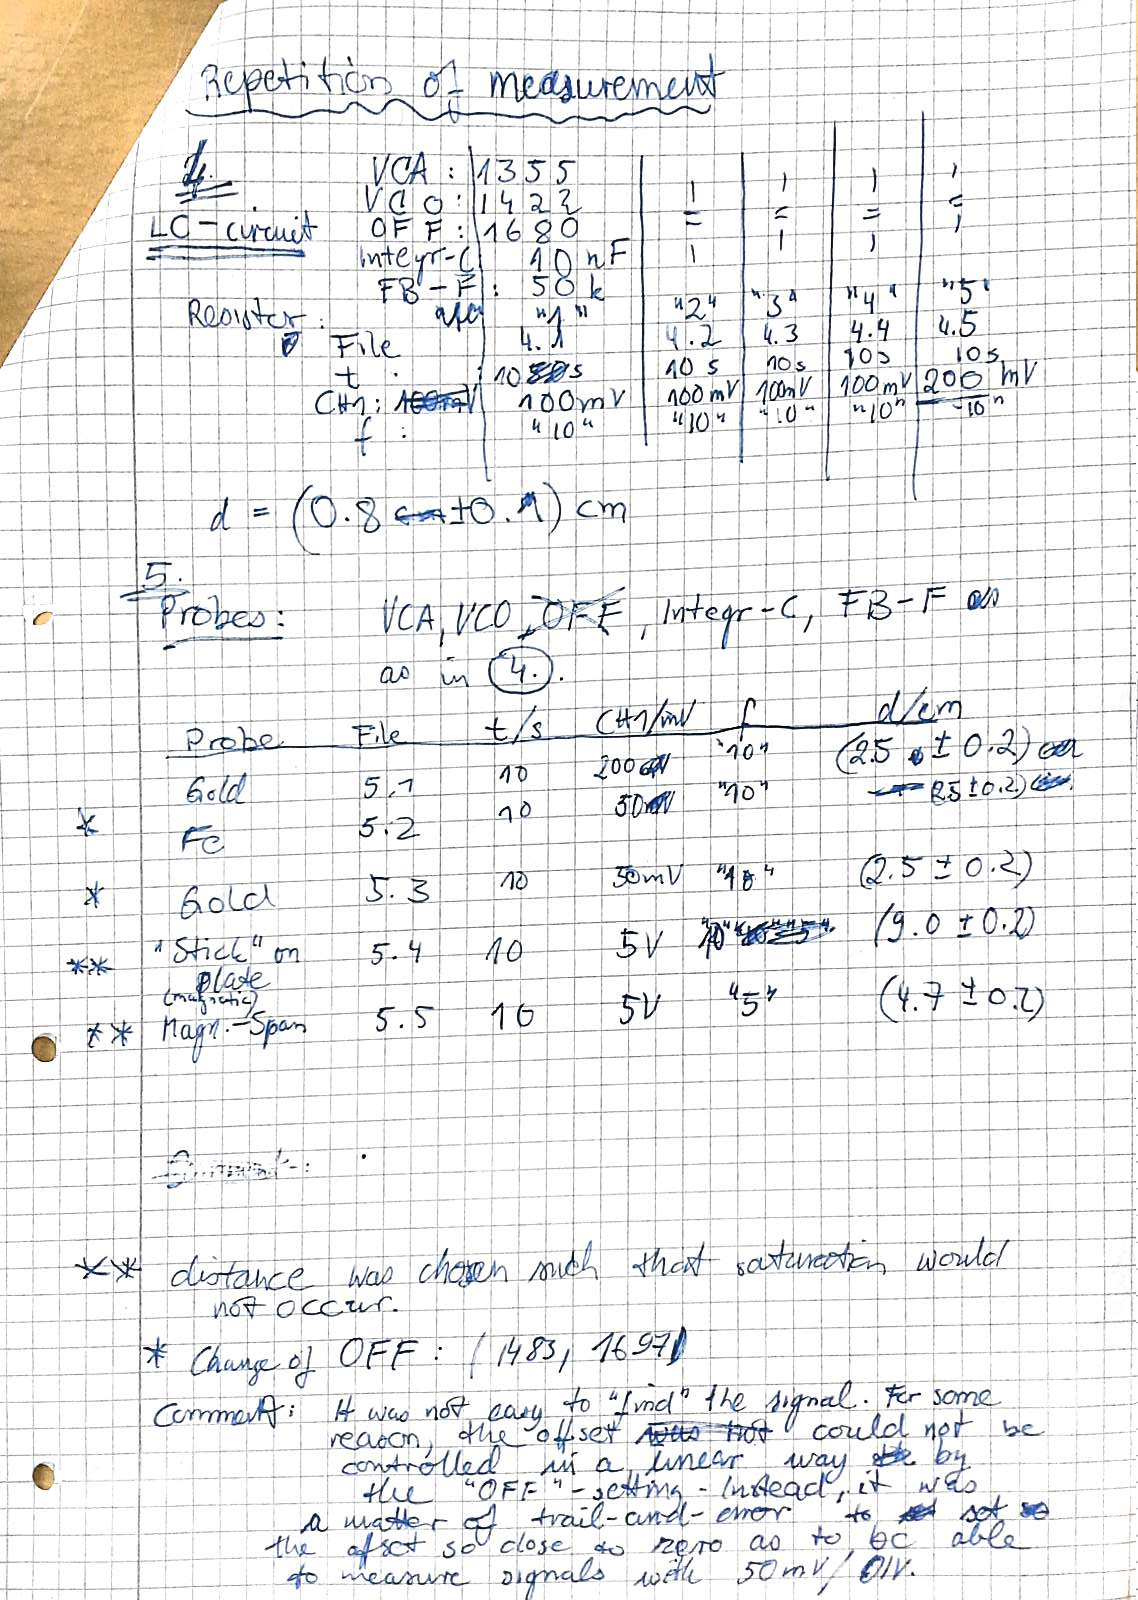
\includegraphics[width=\linewidth]{appendix/page3.jpeg}
\clearpage
\FloatBarrier

